\documentclass[journal]{IEEEtran}

\usepackage{amsmath,amssymb,amsfonts}
\usepackage{graphicx}
\usepackage{booktabs}
\usepackage{array}
\usepackage{xcolor}
\usepackage[hidelinks]{hyperref}
\usepackage{url}

% --- change marking vs main.tex: set \showchangesfalse for a clean manuscript ---
\newif\ifshowchanges \showchangestrue
\newcommand{\NEW}{\ifshowchanges\color{blue}\fi}
\newcommand{\OLD}{\ifshowchanges\color{black}\fi}

% --- Calibratable numbers (grounded in research-notes.md). Update here only. ---
\newcommand{\jpertokEightB}{0.46}      % J / output token, Llama-3 8B, H100, latency-bound (model)
\newcommand{\jpertokSeventyB}{4.0}     % J / output token, Llama-3 70B, H100, latency-bound (model)
\newcommand{\jpertokSixtyfive}{3.8}    % J / output token, LLaMA-65B (model) vs measured 3--4
\newcommand{\embLlamaEightB}{$0.91$\,GWh}      % pre-training energy, Llama-3 8B (1.3M H100-h x 700 W)
\newcommand{\embLlamaSeventyB}{$4.48$\,GWh}    % pre-training energy, Llama-3 70B (6.4M H100-h x 700 W)
\newcommand{\reasoningBlow}{$\sim\!18\times$}  % CoT/reasoning token blow-up (LLMThinkBench)
\newcommand{\jpertokSeventyBthru}{0.45}        % J/token, Llama-3 70B, H100, throughput regime (model)
\newcommand{\jpertokSeventyBmeas}{0.39}        % J/token, Llama-3 70B FP8, H100 (TokenPowerBench, measured)
\newcommand{\multiagentx}{$\sim\!15\times$}    % multi-agent token overhead vs chat (Anthropic)
\newcommand{\crossoverG}{\ensuremath{1.4\times10^{9}}}    % embodied/operational crossover (8B)
\newcommand{\caseEcal}{\ensuremath{9.3\times10^{-2}}}     % multi-agent RAG case-study agentic-eCAL
\newcommand{\caseEnergy}{\ensuremath{2.4\times10^{3}}}    % multi-agent RAG case-study E_W [J]

% --- Option 2 placement analysis (same workflow and eta as the figures) ---
\newcommand{\handoffBits}{$43.2$\,kbit}                 % inter-agent state per invocation
\newcommand{\parityJpb}{\ensuremath{5.0\times10^{-2}}}  % bearer cost at which E_tx = LLM compute
\newcommand{\parityFactor}{\ensuremath{5.0\times10^{4}}}% multiple of a 1e-6 J/b bearer
\newcommand{\parityVolume}{$2.2$\,Gbit}                 % hand-off volume for parity at 1e-6 J/b

\newcommand{\agecal}{\textit{agentic-eCAL}}
\newcommand{\ecal}{\textit{eCAL}}

\begin{document}

\title{Where Should Agents Live? \\Energy Cost of AI Workflows in the Network}

\author{\IEEEauthorblockN{Anonymous Authors}% TODO author block
\thanks{Manuscript draft. }}

\maketitle

\begin{abstract}


We generalize \ecal{} ( Energy Cost of the AI
Lifecycle) from a single AI model lifecycle to an agentic workflow metric \agecal{} quantifying the energy cost of a 
directed graph of LLM calls, tool invocations, retrievals, and inter-agent messages. We derive a
closed-form energy model for a single LLM call from its prefill/decode token-FLOP structure and the
context-dependent attention cost, compose it into a workflow-level energy that captures the
super-linear growth of context in multi-step agent loops, price inter-agent communication with the
OSI transmission model of the original \ecal{}, and amortise the embodied (pre-training) energy of
the open-weight model over its deployment. Calibrated to a single utilization
factor, the single-call model reproduces measured per-token energy across both latency- and
throughput-optimized serving (from $3$--$4$\,J/token for a 65B model in 2023 to sub-J/token for
current open-weight models). A numerical study and a multi-agent retrieval-augmented case study show
that, unlike a one-shot inference, the dominant cost of an agentic workflow is the repeated,
history-carrying generation across steps and agents, and we quantify when retrieval, tool use, and
orchestration overheads matter. \NEW Sweeping that workflow over placements from a single host to
three network hops, and bearers from optical backbone to NB-IoT, we find inter-agent transmission
never exceeds $2\%$ of workflow energy at the modelled utilization: for agentic workloads the
compute--communication trade is
absent by four orders of magnitude, and placement should be decided on latency, privacy and data
residency rather than communication energy.\OLD
\end{abstract}

\begin{IEEEkeywords}
Agentic AI, energy consumption, AI lifecycle, eCAL,
sustainable networks, edge computing, service placement, large language models, open-weight models.
\end{IEEEkeywords}

% ===========================================================================
\section{Introduction}
% ===========================================================================

Agentic artificial intelligence (AI) describes autonomous workflows in which large language models
(LLMs) reason over multiple steps, call tools, retrieve knowledge, and coordinate as multiple
agents. Such workflows are rapidly being embedded into communication networks and the services
they carry. Increasingly these
workflows rely on \emph{open-weight} models that operators can deploy on their own infrastructure,
distributed between user devices, edge sites and the core: a placement problem conventionally treated as an offloading trade between compute and communication energy. Yet the energy cost of such workflows is poorly understood: existing metrics either stop at a single
model inference or ignore the compute entirely. The original \ecal{}
metric~\cite{chou2026ecal} captured
the end-to-end energy of a \emph{single} AI model's lifecycle (i.e. data collection, preprocessing,
training, evaluation, and inference), as a per-bit quantity $[\mathrm{J/b}]$, and showed that the
more a trained model is used, the more energy-efficient each inference becomes as the fixed
development cost is amortised over a growing number of inferences. However, this no
longer describes how a growing class of network AI services are built. Instead, \emph{agentic}
workflows take a large, \emph{pre-trained, open-weight} LLM and orchestrate it typically as directed graph of: model reasoning 
over multiple steps, external tools calls, document retrieval, and cooperation with other agents. Because such workflows are natural candidates for distribution (an agent
close to the user for latency and privacy, an agent in the core for large data corpus access), they inherit
the placement question above, and this paper asks whether the classical answer still holds:
\emph{does
distributing the agents of an LLM workflow across the network cost meaningful energy?} Three
properties make the energy accounting fundamentally different from a single
inference: 
\paragraph{No bespoke training} The model is taken off the shelf; the analogue of \ecal{}'s
  development energy is the model's \emph{embodied} (pre-training) energy, which is enormous but
  shared across all of the model's users.
\paragraph{The unit of work is a workflow, not an inference} A single task triggers a graph of
  many LLM calls, whose prompts \emph{carry the accumulating transcript}, so token volume, and
  hence energy, grows super-linearly in the number of steps.

\paragraph{Heterogeneous components} Tool calls, retrieval (embedding + vector search), and
  inter-agent messages contribute energy outside the LLM itself, some of which is naturally priced
  by the communication-system model already in \ecal{}.

Our contributions are:
\begin{itemize}
\item We introduce \agecal{} as an analytical tool to estimate the energy footprint of modern agentic workflows  by summing LLM-call, tool, retrieval, inter-agent
  transmission, and orchestration energy 
(Sections~\ref{sec:workflow} and \ref{sec:embodied}). \agecal{} is a strict generalization of \ecal{}: it reduces to the inference term of~\cite{chou2026ecal} for a one-shot call.
  
  \item A closed-form energy model for a single LLM call, derived from the standard $\sim\!2N$
  FLOPs-per-token forward accounting plus the context-dependent attention/KV-cache term, mapped to
  energy through achievable hardware throughput and power (Section~\ref{sec:call}).
  
  \item Our results show that i) the dominant cost of an  agentic workflow are the LLM-calls due to the quadratic-in-steps context growth of
  history-carrying agent loops, ii) energy increase with reasoning depth and agent count for history-carrying vs history-free reasoning are superlinear vs linear iii) for a Llama-3 8B the cross-over to inference-dominated cost is at $G\approx\crossoverG$ invocations and iv) the energy cost of communication should not dictate the agent placement policy (Section~\ref{sec:results}).
\end{itemize}

% ===========================================================================
\section{Related Work}\label{sec:related}
% ===========================================================================
\textit{Lifecycle energy metrics.} \ecal{}~\cite{chou2026ecal} introduced a per-bit,
component-resolved view of AI energy spanning the OSI and cloud-computing reference architectures.
We adopt the same per-bit framing and the same transmission/virtualization machinery, and extend the
\emph{development} and \emph{inference} components to agentic LLM workflows.

\textit{LLM inference compute and energy.} The compute of a decoder-only transformer is governed by
a well-established FLOP accounting: a forward (inference) pass costs $\approx 2N$ FLOPs per token and
a full training step $\approx 6N$ (the backward pass being roughly twice the forward), with a
context-dependent attention term that is negligible until the context length exceeds
$\approx 8d$~\cite{kaplan2020scaling,deepmind_scaling_book}. On the measurement side, Samsi
\emph{et al.}~\cite{samsi2023words} report $3$--$4$\,J per output token for LLaMA~65B on V100/A100,
the ML.ENERGY benchmark~\cite{mlenergy2025} shows per-generation energy falling $\sim\!3.5\times$
from batch~4 to batch~64 on H100 and warns that estimating energy from nameplate TDP overestimates
measured energy by up to $4.1\times$, and frontier-scale serving reaches a median $0.31$\,Wh per
query~\cite{oviedo2026joule}. We adopt the $2N$ accounting and calibrate a utilization factor to
these measurements rather than to peak FLOP/s.

\textit{Embodied cost of open-weight models.} Pre-training energy is documented in primary model
cards and peer-reviewed audits: Llama~2 required $3.3$M A100-hours ($539$\,tCO$_2$eq) and Llama~3
$7.7$M H100-hours ($2290$\,tCO$_2$eq, of which $1.3$M\,h for the 8B and $6.4$M\,h for the
70B)~\cite{touvron2023llama2,llama3card}; Luccioni \emph{et al.}~\cite{luccioni2023bloom} decompose
BLOOM-176B's $50.5$\,tCO$_2$eq lifecycle into $\sim\!22\%$ embodied and $\sim\!78\%$ operational.
Crucially, inference only overtakes training at fleet scale, with parity after $\sim\!205$M
(BLOOMz-560M) to $\sim\!593$M (BLOOMz-7B) inferences~\cite{luccioni2024power}, which motivates
amortizing embodied
energy over deployment volume.

\textit{Agentic, reasoning, and RAG systems.} The defining energy property of agentic AI is
\emph{token amplification}: reasoning models emit \reasoningBlow{} more tokens than standard models on
the same task (e.g.\ Phi-4-reasoning-plus $6{,}780$ vs Phi-4 $378$ tokens), sometimes at lower
accuracy~\cite{llmthinkbench2025}, and test-time scaling with $\sim\!15\times$ tokens raises per-query
energy $\sim\!13\times$~\cite{oviedo2026joule}. Because energy scales near-linearly with generated
tokens, this directly multiplies the per-token term. Agent composition compounds it: single agents
use $\sim\!4\times$ and multi-agent systems \multiagentx{} more tokens than a chat
call~\cite{anthropic_multiagent}, and multi-agent debate can reach $32$--$158\times$ a single call
before sparse-communication methods recover much of it~\cite{s2mad2025}. In retrieval-augmented
generation the injected context dominates: a $\sim\!100$-token request plus $\sim\!1000$ retrieved
tokens makes the augmented request $>\!10\times$ costlier~\cite{ragcache2024}, while prefix/KV-cache
reuse of that context cuts time-to-first-token up to $4\times$~\cite{ragcache2024} and tuned RAG
pipelines save up to $60\%$~\cite{ragenergy2026}.
Model choice is a complementary lever: measured per-token energy rises
$\sim\!18\times$ from Llama-3 1B to 70B, so a 1B model costs roughly $5\%$
of a 70B model per generated token~\cite{tokenpowerbench2026},
as is sparsity: Mixture-of-Experts
energy tracks \emph{active} not total parameters, e.g.\ a 30B-A3B model uses $3.56\times$ less
energy/token than a dense 32B~\cite{mlenergy_v3}. Crucially, all agentic/tool evidence is in
\emph{token} units, and no published study measures the joules of a full open-weight agentic run,
so we bridge tokens to energy via the per-token model and flag the tool/orchestration terms as
analytical.

\begin{table}[t]
\caption{Summary of notation.}
\label{tab:notation}
\centering
\small
\begin{tabular}{@{}ll@{}}
\toprule
Symbol & Description \\
\midrule
$N$ & model parameters ($N_{\mathrm{act}}$: active per token, MoE) \\
$n_\ell,\, d$ & number of layers, hidden size \\
$p_{\mathrm{in}},\,p_{\mathrm{out}}$ & prompt (prefill) and generated (decode) tokens \\
$C_{\mathrm{call}}$ & forward FLOPs of one LLM call \\
$\Pi$ & peak FLOP/s of the accelerator \\
$\eta$ & model-FLOP utilization (achieved/peak) \\
$b$ & serving (decode) batch size \\
$c_{\mathrm{pre}},c_{\mathrm{dec}}(b)$ & per-token prefill, decode energy [J/tok] \\
$P$ & board power while busy [W] \\
$E_{\mathrm{call}}$ & energy of one LLM call [J] \\
$K$ & number of workflow steps \\
$h_k$ & carried-history tokens at step $k$ \\
$E_W$ & operational workflow energy [J] \\
$E_{\mathrm{emb}}$ & embodied (pre-training) energy [J] \\
$\gamma_{\mathrm{v}},\,\gamma_{\mathrm{e}}$ & virtualization, embodied-amortization factors \\
$f$ & bits per token \\
\bottomrule
\end{tabular}
\end{table}

% ===========================================================================
\section{Agentic Lifecycle and the Agentic-eCAL Metric}\label{sec:metric}
% ===========================================================================
We consider a communication-and-computing system that serves a task by executing an \emph{agentic
workflow} on a pre-trained open-weight LLM with $N$ parameters. A workflow $W$ is a sequence of
$K$ steps $s_1,\dots,s_K$. Each step is executed by an agent $a(s_k)$ and consists of one LLM call,
optionally preceded by a retrieval and followed by a tool invocation. Following \ecal{}, we express
the metric as the ratio of total energy consumed to the useful application-level data produced:
\begin{equation}
\agecal = \frac{E_W + \gamma_{\mathrm{e}} E_{\mathrm{emb}}}{B_{\mathrm{useful}}} \quad [\mathrm{J/b}],
\label{eq:metric}
\end{equation}
where $E_W$ is the operational energy of the workflow, $E_{\mathrm{emb}}$ is the embodied
(pre-training) energy of the open-weight model, $\gamma_{\mathrm{e}}\in[0,1]$ is the fraction of that
embodied energy attributed to one workflow invocation, and
$B_{\mathrm{useful}} = f\,T_{\mathrm{out}}$ is the useful output measured in bits ($T_{\mathrm{out}}$
useful output tokens at $f$ bits/token). Table~\ref{tab:notation} summarizes the notation.

The operational energy of a workflow $E_{W}$ sums the energy of every component, scaled by a virtualization and system 
orchestration overhead $\gamma_{\mathrm{v}}$ (the same factor \ecal{} uses for cloud platform
overheads, Eq.~(30) of~\cite{chou2026ecal}):
\begin{equation}
E_W = (1+\gamma_{\mathrm{v}})\!\left[\sum_{k=1}^{K} E_{\mathrm{call}}^{(k)} + \sum_{k} E_{\mathrm{tool}}^{(k)} + \sum_{k} E_{\mathrm{ret}}^{(k)} + E_{\mathrm{tx}}^{(k)}\right]
\label{eq:ew}
\end{equation}

\noindent where $E_{\mathrm{call}}^{(k)}$ is the energy of the LLM call at step k, $E_{\mathrm{tool}}^{(k)}$ the execution energy of any tool that step invokes, $E_{\mathrm{ret}}^{(k)}$ the cost of any retrieval preceding it (query embedding plus index search), and $E_{\mathrm{tx}}$ the transmission energy of the messages received from other  agents. At $\!K\!=\!1$ with no tools or retrievaland with co-located agents, $E_W\!\to\!(1{+}\gamma_{\mathrm{v}})E_{\mathrm{call}}$ and
Eq.~\eqref{eq:metric} reduces to \ecal{}'s energy-per-bit of a single inference, with the denominator
specialising \ecal{}'s \emph{manipulated}-data bits to the workflow's \emph{useful output} bits, the
bits it \emph{delivers} rather than those it ingests. \agecal{} is thus a strict generalization of
\ecal{}, adding the multi-call graph on top of the single-inference term.

%===========================================================================
\subsection{Energy of a Single LLM Call}\label{sec:call}
% ===========================================================================
A call has two phases with different energy characteristics.
\emph{Prefill} processes all $p_{\mathrm{in}}$ prompt tokens in one parallel pass, and is \textit{compute-bound} at
near-peak utilization. \emph{Decode} emits $p_{\mathrm{out}}$ tokens one at a time and is
\textit{memory-bandwidth-bound}: each step streams the model weights (and the growing KV-cache) from HBM while
the arithmetic units sit largely idle. Decode is $77$--$91\%$ of inference time and nearly
insensitive to compute clock~\cite{decode_membound2025}We formalize this as a \emph{two-rate} model,
\begin{equation}
E_{\mathrm{call}}(p_{\mathrm{in}},p_{\mathrm{out}};b)\;\approx\;
  c_{\mathrm{pre}}\,p_{\mathrm{in}}\;+\;c_{\mathrm{dec}}(b)\,p_{\mathrm{out}},
\label{eq:tworate}
\end{equation}
with per-prefill-token energy $c_{\mathrm{pre}}$ and per-decode-token energy $c_{\mathrm{dec}}(b)$ at
serving batch size $b$. 


\textit{Prefill} is compute-bound and we model it with  Eq. \ref{eq:pre} where $\eta_{\mathrm{pre}}$ near peak and essentially batch-independent.  

\begin{equation}
c_{\mathrm{pre}}\approx 2N\,P/(\eta_{\mathrm{pre}}\Pi)
\label{eq:pre}
\end{equation}

\textit{Decode} is memory-bound: each
step reads the $\sim\!2N$ weight bytes from HBM \emph{once for the whole batch}, so that cost
amortizes over the $b$ concurrently-decoding sequences,
\begin{equation}
c_{\mathrm{dec}}(b)\;\approx\;\frac{P}{B_{\mathrm{HBM}}}\!\left(\underbrace{\frac{2N\beta}{b}}_{\text{weights}/\text{batch}}
   \;+\;\underbrace{\gamma\,\bar c}_{\text{KV-cache}}\right),
\label{eq:cdec}
\end{equation}
where $B_{\mathrm{HBM}}$ is HBM bandwidth, $\beta$ bytes per parameter, and $\gamma\bar c$ the
per-token KV-cache traffic at mean context $\bar c$. 

Looking at Eq. \ref{eq:tworate}, it can be seen that a call is prefill-dominated when
$c_{\mathrm{pre}}\,p_{\mathrm{in}}>c_{\mathrm{dec}}(b)\,p_{\mathrm{out}}$, that is when
$p_{\mathrm{in}}/p_{\mathrm{out}}>c_{\mathrm{dec}}(b)/c_{\mathrm{pre}}$. At small batch
$c_{\mathrm{dec}}\!\gg\!c_{\mathrm{pre}}$ and energy tracks the \emph{decode} (output) workload. As
$b$ grows, the weight term in Eq.~\eqref{eq:cdec} vanishes, $c_{\mathrm{dec}}(b)$ falls toward the
KV floor, and any workload with $p_{\mathrm{in}}\!\gg\!p_{\mathrm{out}}$ becomes
\emph{prefill}-dominated. This is the agentic regime: because the transcript accumulates, $\sum_k p_{\mathrm{in}}^{(k)}$ grows super-linearly while generated
output grows only linearly, so at production batch sizes the workflow crosses into the
prefill-dominated regime and \agecal{} grows super-linearly, whereas the \emph{same} workflow at
single-stream serving stays linear. 

\subsection{Energy of a Sequence of  LLM Calls}\label{sec:callseq}

In a history-carrying loop the prompt of step $k$
carries the system/tool-schema prompt $p_{\mathrm{sys}}$, any newly introduced tokens, retrieved
context, and the accumulated transcript $h_k=\sum_{j<k}\!\big(p_{\mathrm{out}}^{(j)}+o^{(j)}\big)$
($o^{(j)}$: tool observations). With a fixed emission $s$ per step, $p_{\mathrm{in}}^{(k)}\!\approx\!
p_{\mathrm{sys}}+s\,k$, so the \emph{token} volume is exactly quadratic while the generated output is
linear:
\begin{equation}
\sum_{k=1}^{K} p_{\mathrm{in}}^{(k)} = \tfrac{s}{2}K^2 + O(K),
\qquad
\sum_{k=1}^{K} p_{\mathrm{out}}^{(k)} = sK .
\label{eq:tokgrow}
\end{equation}
Substituting into Eq.~\eqref{eq:ew} through the two-rate model, the operational energy is
\begin{equation}
E_W \;\propto\; c_{\mathrm{pre}}\,\big(\tfrac{s}{2}K^2\big) \;+\; c_{\mathrm{dec}}(b)\,sK ,
\label{eq:ewscale}
\end{equation}
so \agecal{} scales as $K^{a}$ with a \emph{batch-set} exponent $1\!\le\!a\!\le\!2$: at small batch
$c_{\mathrm{dec}}(b)\!\gg\!c_{\mathrm{pre}}$ and the linear decode term dominates ($a\!\to\!1$); as $b$
grows, $c_{\mathrm{dec}}(b)\!\to\!0$ and the quadratic prefill term takes over ($a\!\to\!2$). The
distinction matters: the \emph{context} grows quadratically unconditionally
(Eq.~\eqref{eq:tokgrow}), but the \emph{energy} inherits that growth only when prefill-dominated.


TODO - move to results

which is why the measured exponent (Section~\ref{sec:call}) is $a\!\approx\!1.3$--$1.4$, not $2$,
reflecting partial prefill dominance at the tested batches. The multi-agent \emph{width} axis is
identical: under all-to-all communication each of $N$ agents reads the other $N\!-\!1$, so per-call
input is $\Theta(N)$ and $\sum_k p_{\mathrm{in}}^{(k)}=\Theta(N^2)$, giving the same
$1\!\le\!a\!\le\!2$ law in $N$. Sparser coupling lowers the exponent, and \emph{independent} agents
(no peer context) collapse it to a linear $\Theta(N)$ (the efficient fan-out case). A single crossover
thus governs both reasoning depth ($K$) and team width ($N$). This is the agentic counterpart of
\ecal{}'s amortization: there, lifecycle energy is spread \emph{over} inferences. Here it
\emph{accumulates} within one workflow.

\subsection{Energy of Tool Calls} 
A tool invocation contributes its own execution energy $E_{\mathrm{tool}}^{(k)}$
and injects $o^{(k)}$ observation tokens into the transcript. Non-LLM tools that fetch data over the
network are priced by the OSI data-collection model $E_{DC}$ of \ecal{}~\cite{chou2026ecal}); local compute tools by their FLOPs and the same energy mapping as
Eq.~\eqref{eq:pre}.

\subsection{Energy of Retrieval} 
A retrieval step embeds the query with an embedding model
($\approx 2N_{\mathrm{emb}}\,p_q$ FLOPs for $p_q$ query tokens), searches a vector index of
$M_{\mathrm{vec}}$ vectors of dimension $d_{\mathrm{emb}}$ (cost $\propto d_{\mathrm{emb}}M_{\mathrm{vec}}$
for exact search, or $\propto d_{\mathrm{emb}}\log M_{\mathrm{vec}}$ for graph-based approximate
search)~\cite{HNSW_Malkov2020}, and injects $k_r$ chunks of $L_r$ tokens that enlarge the next
call's prompt. The search compute can be expressed as: 
\begin{equation}
C_{\mathrm{call}}(p_{\mathrm{in}},p_{\mathrm{out}}) = 2N\,n + n_\ell\, d\, n\,(n+1).
\label{eq:ccall}
\end{equation}

\noindent where $N$ is the number of parameters, $n$ is the number of tokens, $n_l$ and $d$ are the number of layers and hidden size. The added context tokens are
captured by
Eqs.~\eqref{eq:tokgrow}. Empirically, growing the context from $2$K to $10$K tokens raises measured energy per token
$\sim\!3\times$ for a $70$B model~\cite{tokenpowerbench2026,sweetspot2026}. 

\subsection{Energy of Multi-agent Communication.} 
When agents are co-located the hand-off cost is just additional
prompt tokens; when distributed, each inter-agent message of $b$ bits incurs transmission energy
priced by the per-layer OSI model of \ecal{}, so $E_{\mathrm{tx}}=\sum_{\text{messages}}E_{\mathrm{DC}}(b)$.

% \begin{table}[t]
% \caption{Summary of notation.}
% \label{tab:notation}
% \centering
% \small
% \begin{tabular}{@{}ll@{}}
% \toprule
% Symbol & Description \\
% \midrule
% $N$ & model parameters ($N_{\mathrm{act}}$: active per token, MoE) \\
% $n_\ell,\, d$ & number of layers, hidden size \\
% $p_{\mathrm{in}},\,p_{\mathrm{out}}$ & prompt (prefill) and generated (decode) tokens \\
% $C_{\mathrm{call}}$ & forward FLOPs of one LLM call \\
% $\Pi$ & peak FLOP/s of the accelerator \\
% $\eta$ & model-FLOP utilization (achieved/peak) \\
% $P$ & board power while busy [W] \\
% $E_{\mathrm{call}}$ & energy of one LLM call [J] \\
% $K$ & number of workflow steps \\
% $h_k$ & carried-history tokens at step $k$ \\
% $E_W$ & operational workflow energy [J] \\
% $E_{\mathrm{emb}}$ & embodied (pre-training) energy [J] \\
% $\gamma_{\mathrm{v}},\,\gamma_{\mathrm{e}}$ & virtualization, embodied-amortization factors \\
% $f$ & bits per token \\
% \bottomrule
% \end{tabular}
% \end{table}

% 




% ===========================================================================
\begin{figure*}[t]
  \centering
  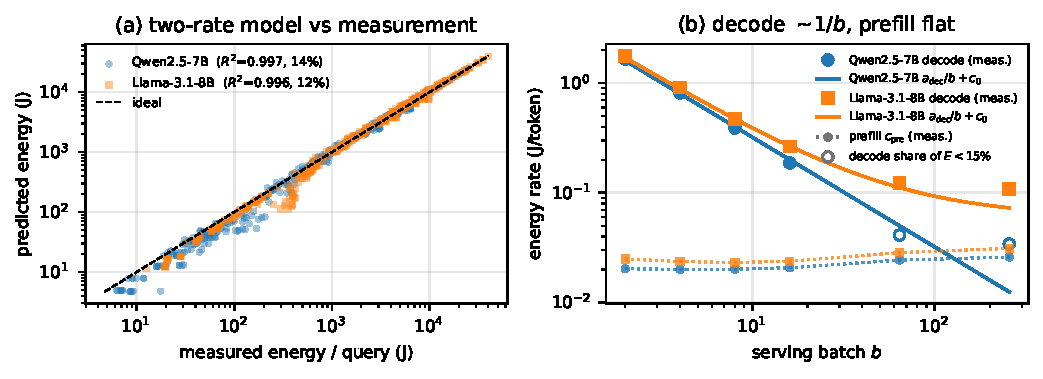
\includegraphics[width=\textwidth]{figures/fig_validation.pdf}
  \caption{Empirical validation of the two-rate model (Qwen2.5-7B and Llama-3.1-8B; A100, vLLM;
  $270$ configurations per model, $2$--$30$ agents, serving batch $b\!\in\![2,256]$, three tasks).
  (a)~Predicted vs.\ measured per-query GPU energy over four orders of magnitude
  ($R^2\!>\!0.99$, mean absolute error ${\sim}10\%$); the residual tail is small-team, high-batch
  calls, where a fixed per-request overhead the model omits becomes visible. (b)~The two rates
  recovered by regressing energy on $(p_{\mathrm{in}},p_{\mathrm{out}})$ at each batch: the prefill
  rate $c_{\mathrm{pre}}$ (dotted) is batch-independent, while the decode rate (markers) collapses as
  $a_{\mathrm{dec}}/b$ toward a small floor (solid lines, Eq.~\eqref{eq:cdec}). Llama's higher floor
  keeps it partly decode-bound at large batch.}
  \label{fig:validation}
\end{figure*}

\begin{table}[t]
\caption{Model vs.\ measured per-output-token energy (validation).}
\label{tab:validation}
\centering
\small
\begin{tabular}{@{}lllll@{}}
\toprule
Model & HW & regime & $E_{\mathrm{call}}$ & measured \\
\midrule
LLaMA-65B   & A100 & latency ($\eta{=}0.05$)    & \jpertokSixtyfive{} & $3$--$4$~\cite{samsi2023words} \\
Llama-3 70B & H100 & throughput ($\eta=0.25$) & 0.45 & 0.69~\cite{tokenpowerbench2026} \\
Llama-3 8B  & H100 & throughput ($\eta=0.25$) & 0.05 & 0.11~\cite{tokenpowerbench2026} \\
% NOTE(Qwen model identity): [18]'s prose says "Qwen 8B, 32B and 480B" and its Fig. 3
% x-axis prints "Qwen-8B", but its released code names the weights explicitly. The
% TokenPowerBench repo (github.com/chenxuniu/TokenPowerBench), README "Required
% Models", downloads Qwen/Qwen2.5-7B-Instruct, Qwen2.5-32B-Instruct and
% Qwen2.5-72B-Instruct -- no Qwen3 anywhere. So [18]'s "Qwen-8B" is Qwen2.5-7B and the
% figure label's size digit is wrong (the same slip appears as "Falcon-10B", where the
% repo downloads falcon-40B and falcon-7B). We therefore name the actual model, which
% is also the model of Fig. 2. Geometry from the HF config: 7.615e9 params, 28 layers,
% d=3584 -> 0.049 J/token, printed 0.05.
% Measured value read from Fig. 3(b) of [18] (GPU panel, 0-2K band): 0.111.
% Qwen2.5-32B (measured 0.593, modelled 0.21) was considered and dropped: [18] never
% states whether the 32B was sharded, so the idle-sibling correction below cannot be
% applied to it.
\NEW{}Qwen2.5-7B  & \NEW{}H100 & \NEW{}throughput ($\eta=0.25$) & \NEW{}0.05 & \NEW{}0.11~\cite{tokenpowerbench2026} \\
\bottomrule
\multicolumn{5}{l}{\footnotesize Units: J per output token. \NEW{}Model: $p_{\mathrm{in}}{=}64$, $p_{\mathrm{out}}{=}512$. Measured: GPU-only,} \\
\multicolumn{5}{l}{\footnotesize \NEW{}$0$--$2$K context band, Fig.~3(b) of~\cite{tokenpowerbench2026} ($4{\times}$H100 node). The 7B and 8B} \\
\multicolumn{5}{l}{\footnotesize \NEW{}runs occupy one GPU, so ${\sim}38\%$ of their value is idle sibling draw ($\approx\!0.07$);} \\
\multicolumn{5}{l}{\footnotesize \NEW{}the 70B is sharded over all four.}
\end{tabular}
\end{table}

% ===========================================================================
\subsection{Amortized Embodied Cost of Open-Weight Models}\label{sec:embodied}
% ===========================================================================
\ecal{} amortizes a model's one-time development energy $E_{\mathrm{D}}$ over the number of
inferences served. For an open-weight model the development cost is the \emph{pre-training} energy
$E_{\mathrm{emb}}$, which is incurred once by the model producer but shared across \emph{all}
downstream deployments. If a model serves $G$ workflow invocations over its deployed lifetime, the
embodied energy attributable to one invocation is $\gamma_{\mathrm{e}}E_{\mathrm{emb}}$ from Eq. \ref{eq:metric} with  $\gamma_{\mathrm{e}}=1/G$. As with \ecal{}'s amortization-over-inferences result, this share
vanishes at scale, so for widely served open-weight models the operational term $E_W$ dominates
\agecal{}. The crossover point (how many invocations are needed before operation overtakes embodied cost) depends on $E_{\mathrm{emb}}$ and is reported in Section~\ref{sec:results}.

\section{Numerical Analysis and Case Study}\label{sec:results}
% ===========================================================================

\subsection{Experimental Validation of the LLM Call Energy Model} 

We treat the multi-agent workflow as a controllable dial on
input-token volume: varying agents and steps grows the accumulating context $p_{\mathrm{in}}$
super-linearly at near-linear output (Eq.~\eqref{eq:tokgrow}), and we fit GPU energy (metered by NVML)
to the resulting $(p_{\mathrm{in}},p_{\mathrm{out}})$ counts via Eq.~\eqref{eq:tworate}, so only token
volume enters the model, not the task. On Qwen2.5-7B and Llama-3.1-8B (NVIDIA A100, vLLM continuous
batching), across team sizes of $2$ to $30$ agents per task and batch (GPQA, GSM-Hard, MMLU-Hard;
$R^2\!>\!0.99$, mean absolute error ${\sim}10\%$; Fig.~\ref{fig:validation}) this recovers the two rates on each: a near-constant $c_{\mathrm{pre}}\!\approx\!0.02$--$0.03$\,J/token
(the compute-bound prefill floor) and a decode rate that collapses $\sim\!1/b$ ($p\!<\!0.001$). Both
rates match first principles: $c_{\mathrm{pre}}$ implies a prefill utilization $\eta_{\mathrm{pre}}\!\approx\!0.64$
(compute-bound, as expected), and the decode coefficient agrees with the memory-bandwidth prediction
$PN\beta/B_{\mathrm{HBM}}$ to within $10\%$. The energy-vs-agent-count exponent rises with batch
accordingly, from $a\!\approx\!1.10$ to $1.42$ for Qwen ($b\!:\!2\!\to\!256$) and from $1.02$ to
$1.17$ for Llama, a direct GPU-energy measurement that confirms the predicted super-linear,
batch-dependent crossover. The milder Llama slope reflects the crossover directly: a
higher decode floor ($c_{\mathrm{dec}}\!\approx\!0.06$ vs ${\sim}0.02$ at $b\!=\!256$) keeps it partly
decode-bound, so architecture sets how far the workflow crosses. As an independent
cross-hardware check, the single-rate special case reproduces measured per-token energy at both
utilization extremes (Table~\ref{tab:validation}): \jpertokSixtyfive{}\,J/token for LLaMA-65B at
latency-bound $\eta{=}0.05$ (measured $3$--$4$~\cite{samsi2023words}) and \jpertokSeventyBthru{}\,J/token
for Llama-3~70B at throughput-optimized $\eta{=}0.25$ (measured \jpertokSeventyBmeas{}, FP8~\cite{tokenpowerbench2026}).
Serving choices (batch size, quantization, KV-cache reuse) move $c_{\mathrm{dec}}(b)$ and hence the
crossover, which the two-rate model makes explicit.

\begin{figure*}[t]
  \centering
  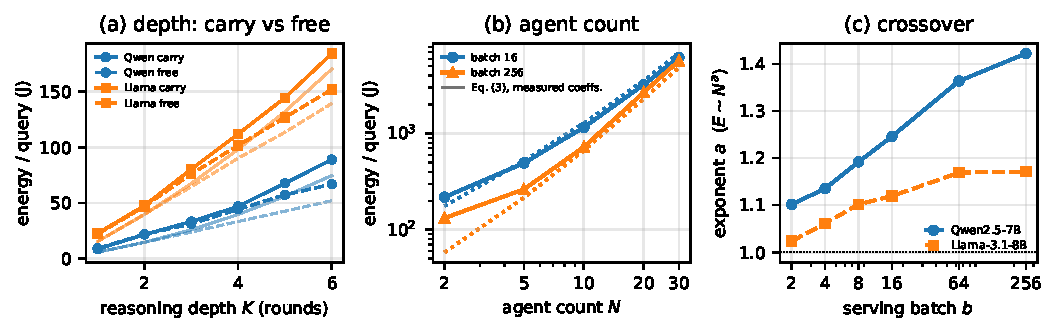
\includegraphics[width=\textwidth]{figures/fig_scaling.pdf}
    \caption{Measured scaling (A100, vLLM). (a) Reasoning depth on Qwen2.5-7B\NEW{} and
  Llama-3.1-8B\OLD{}: per-query energy vs.\
  rounds, history-carrying vs.\ history-free. (b) Agent count on Qwen2.5-7B: energy vs.\ $N$ at a
  small and a large serving batch. (c) The energy-vs-agent-count exponent $a$ rises with batch on
  both Qwen2.5-7B and Llama-3.1-8B: the prefill/decode crossover. 
 \NEW{}Grey lines in (a) and (b):
  \ecal{} evaluated on the same measured token workload at $\eta=0.25$, $0.5$, $0.75$ and $1$
  (A100 nameplate power), $\eta=1$ being the peak-FLOP floor.\OLD{} Panel (c) carries no model line, as
  $\eta$ cancels from a log--log slope. }

  \label{fig:scaling}
\end{figure*}

\subsection{Experimental Validation of Scaling the Call Energy Model} Because decode is memory-bound, the achieved utilization
$\eta$ spans roughly $0.05$ (single-stream, latency-bound \NEW{}decode\OLD{}) to \NEW{}$\sim\!0.7$
(prefill-dominated work at large batch): decode streams the weights once per generated token, while
prefill is a single batched matmul and is compute-bound\OLD{}. The lower end is
consistent with the batch-size swing measured in~\cite{mlenergy2025}\NEW{}, the upper end with the
utilization overlays of Fig.~\ref{fig:scaling}\OLD{}.
We calibrate $\eta$ to measured energy rather than peak FLOP/s, since nameplate thermal design power  overestimates
measured energy by up to $4.1\times$: decode is memory-bandwidth-bound and underutilizes the GPU's
compute~\cite{mlenergy2025,decode_membound2025}. Concretely, decode accounts for $77$--$91\%$ of
inference time and is nearly insensitive to GPU compute clock~\cite{decode_membound2025}; $\eta$ thus
folds in this memory-bound behaviour. Table~\ref{tab:validation} shows the model tracks measured per-token energy across an
order of magnitude in model scale and both ends of the $\eta$ range. At $\eta=0.05$
(latency-bound) it yields $3.8$\,J/token for LLaMA-65B, matching the $3$--$4$\,J/token
of~\cite{samsi2023words}. At $\eta=0.25$ (throughput-optimized) it yields $0.45$ and
$0.05$\,J/token for Llama-3~70B and~8B against measured $0.69$ and
$0.11$\,J/token~\cite{tokenpowerbench2026}; \NEW{}all three under-estimate by a similar factor\OLD{},
consistent with $\eta=0.25$ being an optimistic ceiling: the 70B measurement implies
$\eta\approx0.16$, within the range the model spans.  Serving choices move energy per
token without changing the model math, which is exactly what $\eta$ captures: batch
size can unlock a $3$--$5\times$ reduction~\cite{mlenergy_v3}, and latency-constrained
Pareto configs save up to $44\%$~\cite{mlenergy2025}.



\subsection{Energy of a Centralized RAG Workflow}
The LLM-call term (Section~\ref{sec:call}) is grounded in measured per-token
energy. The overall workflow's \emph{token} drivers are corroborated by measurement: multi-agent
overhead ($\sim\!4$--$15\times$~\cite{anthropic_multiagent}), RAG context dominance
($>\!10\times$~\cite{ragcache2024}). However, no published study reports the \emph{joules} of a full
open-weight agentic run, the token share of tool schemas/observations, or the energy of failed-call
retries; those tool/orchestration terms therefore remain \emph{analytical} estimates that bridge
tokens to energy via the per-token model, pending direct measurement.

\begin{figure*}[t]
  \centering
  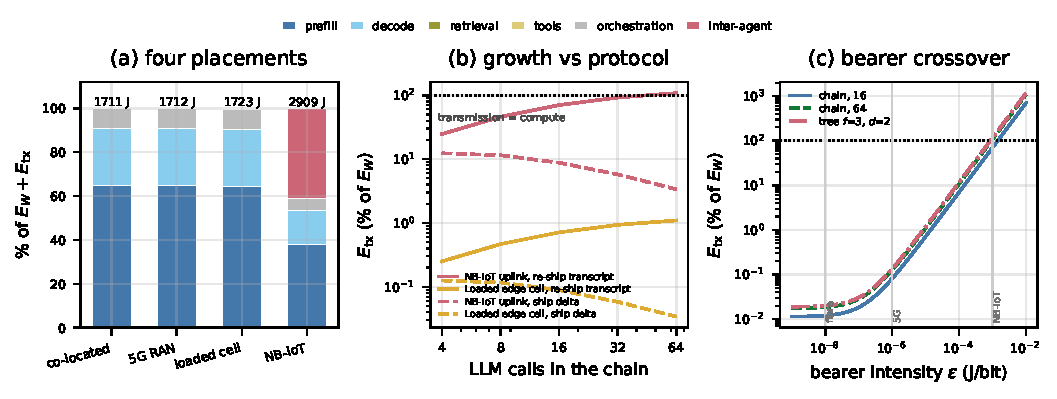
\includegraphics[width=\textwidth]{figures/fig_components.pdf}
    \caption{\ROOF{}Composition of workflow energy against loop depth, at three serving batches.
  The four-agent RAG team is re-run over its own transcript for $K=1\dots6$ rounds, the depth
  range the measured sweeps cover; calls are priced with Eq.~\eqref{eq:tworate} using the measured
  coefficients of Fig.~\ref{fig:validation}, so the prefill and decode bands are its two terms.
  The black curve is total $E_W$ on the right-hand axis, on one scale across all three panels.
  Batch and depth move the composition in the same direction and independently: at single-stream
  serving the workflow is $87\%$ decode, because the weight read is amortised over nothing; at
  batch $256$ it is already $58\%$ prefill at $K=1$. Within every panel prefill then climbs as the
  transcript accumulates---$3.6$ to $11\%$ single-stream, $49$ to $73\%$ at batch $64$. A workflow
  that is decode-bound when serving one user is therefore prefill-bound in production, and
  deepening the loop pushes it further that way at any batch.\OLD{}}
  \label{fig:components}
\end{figure*}


\begin{figure}[t]
  \centering
 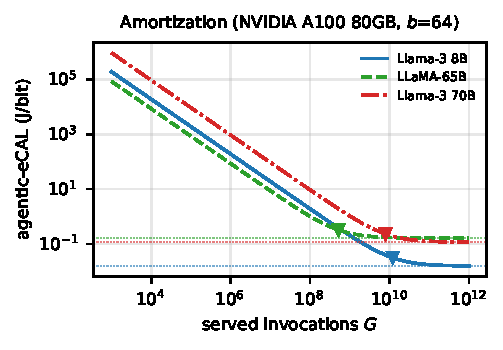
\includegraphics[width=0.88\columnwidth]{figures/fig_amortization.pdf}
  \caption{Embodied vs.\ operational \agecal{} as a function of served invocations $G$ for
  Llama-3 8B; the crossover at $G\approx\crossoverG$ marks where operation overtakes amortized
  pre-training. \NEW{}LLaMA-65B~\cite{touvron2023llama2} and Llama-3~70B are added for comparison,
  all three on the H100 at $\eta=0.05$, as in the case study; the crossover \emph{ratios} between
  models are independent of hardware and $\eta$ alike. Both larger models cross \emph{earlier}
  than the 8B, because pre-training energy grows more slowly than per-invocation energy does.
  Qwen2.5-7B is omitted, its pre-training compute being undisclosed.\OLD{}}
  \label{fig:amortization}
\end{figure}

We instantiate the model on open-weight Llama-3 8B and 70B served on an NVIDIA H100, \NEW{}at the
single-stream, latency-bound utilization $\eta=0.05$: a placement study spans device, edge and core
sites, where an agent serving one user at a time is not batched, so the latency-bound regime applies
rather than the throughput anchor used for the validation in Table~\ref{tab:validation}.\OLD{} All
numbers are produced by the
open-source companion implementation\footnote{\texttt{agentic\_ecal.py}, GitHub link omitted for double blind review}; bits per useful token are taken as
$f=16$\NEW{}, the information-theoretic capacity $\log_2|V|$ of a token drawn from the
$32$k--$128$k vocabularies of the open-weight models considered~\cite{touvron2023llama2,llama3card}\OLD{}.


\textbf{Component breakdown.} Fig.~\ref{fig:components} shows that the LLM calls dominate the energy
of a four-agent RAG workflow (\NEW{}$\sim\!90\%$\OLD{}), followed by the orchestration/virtualization overhead
($\gamma_{\mathrm{v}}$, $\sim\!9\%$); retrieval, tool, and inter-agent transmission energy are
negligible \emph{unless} a tool itself performs heavy computation. The practical implication is that
agentic energy is overwhelmingly \emph{generated- and processed-token} energy, which is exactly the
quantity token amplification inflates.

\ROOF{}Which of the two token classes carries that energy is not fixed, however, and
Fig.~\ref{fig:components} separates the two things that move it. Serving batch sets the starting
point: at single-stream the workflow is $87\%$ decode, because each generated token pays the whole
weight read, whereas at batch $256$ that read is amortised over the batch and the same workflow
begins $58\%$ prefill. Loop depth then moves it further in the same direction at any batch, since
the transcript accumulates while generated output does not---prefill climbs from $3.6\%$ to $11\%$
single-stream and from $49\%$ to $73\%$ at batch $64$ over six rounds. A workflow profiled on one
user is therefore a poor guide to the same workflow in production: it is decode-bound in the first
case and prefill-bound in the second, which inverts what is worth optimising. Absolute energy moves
the other way, batching cutting $E_W$ roughly $14\times$ at every depth, so the two effects must be
read together.\OLD{}


\textbf{Scaling.} Fig.~\ref{fig:scaling} shows the measured scaling against reasoning depth (carry
vs.\ free), agent count, and serving batch. \NEW{}The overlays locate the measurements in $\eta$:
these sweeps are prefill-dominated ($p_{\mathrm{in}}\!:\!p_{\mathrm{out}}\approx20\!:\!1$), so they
sit between $\eta=0.5$ and $\eta=1$, well above the decode-dominated shape of
Table~\ref{tab:validation}.\OLD{} The decisive effect is history carry: accumulating the transcript across steps grows \agecal{}
super-linearly at production batch, while a history-free loop of the same length grows only linearly.
The carry-minus-free exponent gap ($\sim\!0.15$ on Qwen2.5-7B, $\sim\!0.08$ on Llama-3.1-8B) isolates
this accumulation cost. \NEW{}At small batch the exponent falls toward unity (decode-bound), as
Fig.~\ref{fig:scaling}(c) shows.\OLD{} The same accounting subsumes \emph{reasoning} models: a chain-of-thought is additional
\emph{generated} tokens, \NEW{}entering $C_{\mathrm{call}}$ through $p_{\mathrm{out}}$ in
Eq.~\eqref{eq:ccall}\OLD{}, so a
long trace merely shifts the per-call workload toward the decode-bound regime. Whether the surplus tokens are spent as decode (reasoning traces) or, once carried,
re-read as prefill (history), they consume energy without enlarging the useful-output
denominator, the per-bit signature of the \reasoningBlow{} token amplification reported for reasoning
models~\cite{llmthinkbench2025}.

\begin{figure*}[t]
  \centering
  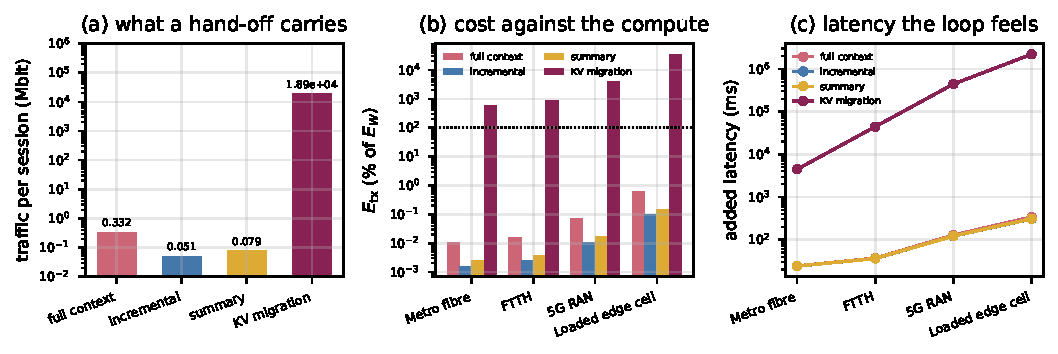
\includegraphics[width=\textwidth]{figures/fig_comm.pdf}
  \caption{\ROOF{}Communication-efficient distributed reasoning. Four hand-off protocols carry the
  same conversation between the same four agents over $K=3$ rounds, on the links of
  Table~\ref{tab:placement} other than the NB-IoT uplink. (a) Traffic per session: re-shipping the
  accumulated context costs $6.5\times$ an incremental hand-off, and migrating the key-value cache
  costs $5.7\times10^{5}$ times as much. (b) The resulting energy relative to the compute it
  accompanies; the dotted line marks parity. (c) The latency the loop incurs. Text-carrying
  protocols remain below $0.7\%$ of workflow energy on every link, whereas cache migration exceeds
  the compute by two to four orders of magnitude and is feasible only over datacentre
  interconnect.\OLD{}}
  \label{fig:comm}
\end{figure*}

\subsection{Communication Energy of a Distributed RAG Workflow}  \NEW The workflow above is a natural candidate for
distribution, so we place it three ways (co-located on a single host, split once between edge and
core, and fully distributed over three hops) and price the hand-offs with the OSI transmission
model of Section~\ref{sec:workflow}. Across agent boundaries it carries $200$, $900$ and $1600$
transcript tokens, i.e.\ \handoffBits{} of inter-agent state per invocation. \NEW{}The workflow
itself consumes $E_W\approx\caseEnergy$\,J, generating $1{,}600$ useful output tokens from $7{,}720$
prefill tokens, a $4.8{:}1$ ratio.\OLD{} Table~\ref{tab:placement} sweeps the bearer cost $\varepsilon$ from an optical backbone to an NB-IoT uplink. Fully
distributing the workflow over a typical 5G bearer raises \agecal{} by $0.002\%$ (four orders of
magnitude below the variation induced by ordinary serving choices such as batch size), and even
three hops over a constrained NB-IoT uplink, which no operator would use to carry agent state,
reaches only $2\%$. \NEW{}These shares scale with $\eta$: at the throughput-optimized $\eta=0.25$ of
Table~\ref{tab:validation} the same three-hop NB-IoT case reaches $\sim\!9\%$, still four orders of
magnitude short of parity.\OLD{} \NEW{}On the fixed and core rows this over-charges transmission:
an already-lit router draws essentially the same power whether or not it carries the
packet~\cite{jacob2025routers}, so the incremental cost of a hand-off there is well below
$\varepsilon$; the mobile rows carry no such slack, a radio drawing power while it transmits.\OLD{}
\ROOF{}Fig.~\ref{fig:comm} isolates the choice that governs this cost, which is the
hand-off protocol rather than the bearer or the topology. A distributed agent requires the state
its predecessor accumulated, and four mechanisms are available for supplying it. Re-shipping the
accumulated context, as a stateless endpoint must, transmits $0.33$\,Mbit per session; carrying
only the increment produced since the recipient last observed the conversation transmits
$0.051$\,Mbit, a factor of $6.5$; a bounded running summary lies between the two. Migrating the
key-value cache instead of reconstructing it transmits $18.9$\,Gbit, five orders of magnitude
above the transcript, because the cache of a single token occupies $131$\,kB against the $17$ bits
of the token itself. The consequences separate sharply. All three text-carrying protocols remain
below $0.7\%$ of workflow energy on every link considered and add at most $339$\,ms; cache
migration exceeds the compute by two to four orders of magnitude and adds $2.2\times10^{3}$\,s on
a loaded cell, confining it to datacentre interconnect. Communication efficiency in a distributed
agentic deployment is therefore obtained at the protocol layer, and the available margin is a
factor of six rather than a matter of bearer selection.\OLD{}


Solving $E_{\mathrm{tx}}=\sum_k E_{\mathrm{call}}^{(k)}$ quantifies the margin:
transmission equals compute only at $\varepsilon\approx\parityJpb$\,J/b, some \parityFactor{} times a
typical mobile bearer, or equivalently if each invocation shipped \parityVolume{} of state instead
of \handoffBits{}. For agentic workloads the compute--communication trade that governs classical
offloading is therefore not merely tilted; it is absent by four orders of magnitude, so agent
placement should be decided on latency, privacy, data residency and corpus locality, and the
energy
budget spent instead on the prefill discipline that Fig.~\ref{fig:scaling} identifies.

\begin{table}[t]
\caption{Inter-agent transmission as a share of workflow energy, by placement and bearer.}
\label{tab:placement}
\centering
\small
\begin{tabular}{@{}lrrr@{}}
\toprule
Bearer ($\varepsilon$ [J/b]) & co-located & $1$ hop & $3$ hops \\
\midrule
Optical backbone ($10^{-8}$)~\NEW{}\cite{vanheddeghem2012}\OLD{}   & $0$ & $<0.001$\% & $<0.001$\% \\
Metro / fixed ($10^{-7}$)~\NEW{}\cite{lorincz2025ftth}\OLD{}       & $0$ & $<0.001$\% & $<0.001$\% \\
5G RAN ($10^{-6}$)~\NEW{}\cite{xu2020operational}\OLD{}            & $0$ & $0.0001$\% & $0.002$\% \\
Loaded edge cell ($10^{-5}$)~\NEW{}\cite{xu2020operational}\OLD{}  & $0$ & $0.002$\%  & $0.020$\% \\
NB-IoT uplink ($10^{-3}$)~\NEW{}\cite{michelinakis2020nbiot}\OLD{} & $0$ & $0.147$\%  & $1.953$\% \\
\bottomrule
% NOTE(bearer energies): epsilon is LINK POWER DIVIDED BY ACHIEVED THROUGHPUT (P_T/R_T + P_R/R_R
% plus OSI processing), the quantity eCAL's transmission model computes. THREE quantities must be
% kept apart, and they span ~7 orders for a core hop:
%   true marginal dP/dr        ~0 (a few pJ/bit; Jacob et al. IMC'25 measure the slope directly)
%   link power / throughput    ~1e-8 J/b   <-- THIS is epsilon
%   network-average intensity  ~1e-4 J/b   (kWh/GB: Pihkola, GSMA, Aslan)
% Do NOT call epsilon "marginal": on an already-lit path the marginal cost of a bit is
% statistically indistinguishable from zero. See bearer-energy-research.md.
% ANCHORS, checked against the sources verbatim:
%  5G  1e-6  : Xu et al. SIGCOMM'20 Fig. 22, y-axis "Efficiency (uJ/bit)"; text says "the
%              energy-per-bit of 5G is only 1/4 of 4G" -> ~5e-7 J/b READ OFF THE AXIS (the
%              number is not in their text). Measured at RSRP [-80,-60] dBm, i.e. good coverage.
%  1e-5      : same source, same measurement outside that window -- Xu state that "poor wireless
%              channel degrades the bit-rate ... which increases the energy per bit", and since
%              eps = power/throughput a ~10x bit-rate drop gives ~10x eps. No separate citation.
%  NB-IoT 1e-3: Michelinakis et al. Table VI, "sending 20 bytes with RAI under good coverage":
%              0.11-0.33 J -> 6.9e-4 to 2.1e-3 J/b. NOTE their 0.82 J figure is Table IV,
%              "includes samples of all packet sizes", NOT a 20 B number -- do not attribute it
%              as such. They also find packet size has "negligible impact" by default, so per-bit
%              normalisation of NB-IoT is loose: energy is connection overhead, not payload.
%  1e-8      : Van Heddeghem et al. Eq. (1) PROPOSE "a simplified IP/MPLS layer power value that
%              expresses the power P_IP of the node based on the total node capacity C_IP:
%              P_IP/C_IP = 10 W/Gbps", set above the CRS-3's achievable 5.5-7.5 W/Gbps because it
%              "seems more reasonable as it implicitly covers sub-optimally filled configurations"
%              -- the same under-filling THIS table's convention prices by dividing by ACHIEVED
%              throughput. 10 W/Gbps = 1.0e-8 J/b exactly: right bearer (IP/MPLS core node), right
%              normalisation, row value on the nose. Two caveats:
%              (a) it is a REFERENCE value, not a measurement. Hence the note says "the backbone
%              row is a reference value, the others measured" -- the distinction must stay on the
%              page, since the inline [n] on the row alone cannot convey it.
%              (b) 2012 (CRS-3 era) and normalised by CAPACITY -- the authors warn efficiency
%              values are "calculated with respect to the capacity of the relevant equipment and
%              not the actual throughput, which could be (far) less". So at real utilisation eps
%              is HIGHER than 1e-8, while newer gear pushes it lower (their own Table 2: 400G
%              ports 1.4 W/Gbps, 1T ports 1.1 W/Gbps; modern coherent optics ~0.05 W/Gbps, i.e. a
%              line-rate hop today is nearer 1e-10). The row is <0.001% in every cell, so neither
%              direction moves the argument.
%              Deep research refuted calling this figure MARGINAL per-hop forwarding energy -- it
%              is not, see the three-way split above -- but did NOT refute the value under the
%              link-power/achieved-throughput convention, which is the one declared here.
%              Corroboration at the same decade, deliberately NOT the row's source: Liu & Choi
%              Sec. 6.2.4 QUOTE J/bit directly -- "the energy (in Joule) consumed to transmit or
%              receive one bit" -- measuring TX 5.1 nJ/bit (single user) to 30 nJ/bit (8MU OFDMA),
%              Fig. 13 axes in nJ/bit, i.e. 5.1e-9 to 3.0e-8 J/b. A WLAN is not a backbone, so it
%              is recorded here only and no longer cited in the table.
%  1e-7      : Lorincz et al. Table 1 measure entire ONU device power at 6-15 W; at 100 Mb/s
%              achieved that is 6e-8 to 1.5e-7 J/b, bracketing the row. Their Table 2 gives GPON
%              ~15-25 W/(Gbit/s)/user (= 1.5-2.5e-8 J/b) and Sec. 3.2 quotes "0.03 uJ/bit at
%              100 Mb/s"; the latter is quoted via their ref [32], so the device-power route is
%              preferred here -- it applies THIS table's own convention to a measured power.
%  (rejected) : a "1.8e-8 J/b core hop" was derived here from
%              Jacob et al. (2.2 kW = ~10% of network power -> 22 kW, over ~1.2 Tbps) and REJECTED:
%              (a) that is network-power/network-traffic, i.e. the network-average category this
%              note tells the reader eps is not; (b) the paper's own "5.9 W = 0.02% of total"
%              implies 29.5 kW instead of 22 kW, a 34% inconsistency; (c) no J/bit figure appears
%              anywhere in Jacob et al. A link-granular route from their per-port terms lands
%              nearer 1e-9. Jacob is cited only for the load-independence of router power.
%              Also rejected as backbone proxies, however close the magnitude: Wi-Fi 6 (a WLAN)
%              and GPON (optical ACCESS, not core). Wrong bearer beats right decade here.
\multicolumn{4}{@{}l}{\footnotesize \NEW{}$\varepsilon$ is link power divided by achieved throughput. The backbone row} \\
\multicolumn{4}{@{}l}{\footnotesize \NEW{}is a reference value, the others measured; the edge row is~\cite{xu2020operational}} \\
\multicolumn{4}{@{}l}{\footnotesize \NEW{}outside its good-coverage window.} \\

\end{tabular}
\end{table}
\OLD

\subsection{Amortization.} Fig.~\ref{fig:amortization} sweeps the number of served invocations $G$. The
embodied (pre-training) energy of Llama-3~8B (\embLlamaEightB{}, i.e.\ $1.3$M H100-hours) dominates
\agecal{} until $G\approx\crossoverG$ invocations, beyond which the operational term sets a floor.
This crossover is the agentic counterpart of \ecal{}'s amortization-of-development-over-inferences
result, and \NEW{}it sits a factor of $\sim\!2$ above the $2$--$6\times10^{8}$\OLD{} inference parity reported
empirically for BLOOMz~\cite{luccioni2024power}. \NEW{}Larger models cross \emph{sooner}, not later:
Llama-3~70B reaches it at $0.57\times$ the 8B's crossover and LLaMA-65B at $0.06\times$, ratios that
are independent of hardware and $\eta$. Pre-training energy grew only $4.9\times$ from the 8B to the
70B while per-invocation energy grows with parameter count, and LLaMA-65B saw $1.4$T training tokens
against Llama-3's $15$T.\OLD{}






\begin{figure*}[t]
  \centering
  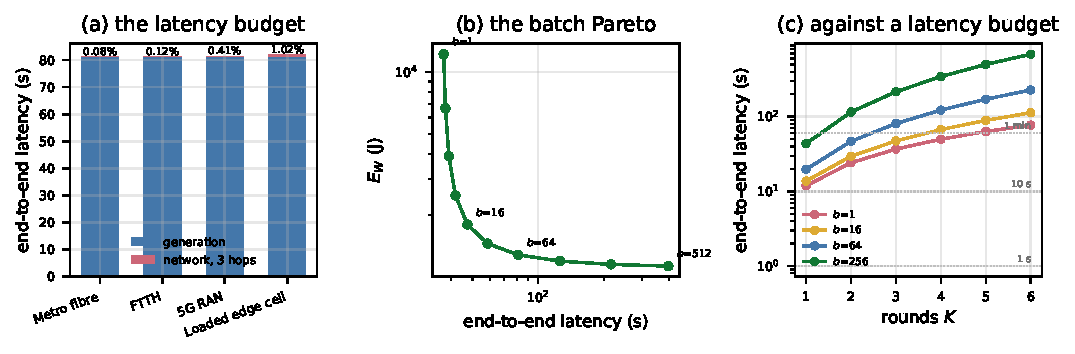
\includegraphics[width=\textwidth]{figures/fig_latency.pdf}
  \caption{\ROOF{}The latency budget of a distributed agentic loop. (a) End-to-end time for the
  four-agent workflow at $K=3$ and $b=64$, decomposed into generation and the network carrying its
  eleven hand-offs over three hops; the network contributes between $0.08\%$ and $1.02\%$ across
  the links of Table~\ref{tab:placement}. (b) The trade that is available: serving batch, over
  which energy falls $10.8\times$ while latency rises $10.7\times$. (c) End-to-end time against
  loop depth at four batches, with reference budgets marked.\OLD{}}
  \label{fig:latency}
\end{figure*}

\ROOF{}% Generated by scripts/clean/make_figures.py -- do not edit by hand.
\begin{table}[t]
\caption{Site dimensioning for an agentic service. One accelerator serving at batch
$64$ completes $0.79$ sessions per second.}
\label{tab:dimensioning}
\centering
\small
\setlength{\tabcolsep}{4pt}
\begin{tabular}{@{}lrrrrrl@{}}
\toprule
 & traffic & load & \multicolumn{3}{c}{accelerators per link} & binding \\
\cmidrule(lr){4-6}
Hand-off protocol & [Mbit] & [Mb/s] & 1\,GbE & 10\,GbE & 100\,GbE & resource \\
\midrule
full context & 0.332 & 0.261 & 3,825 & 38,246 & 382,456 & compute \\
incremental & 0.051 & 0.0402 & 24,860 & 248,597 & 2,485,965 & compute \\
summary & 0.079 & 0.0624 & 16,038 & 160,385 & 1,603,849 & compute \\
KV migration & 1.89e+04 & 1.49e+04 & 0.07 & 0.67 & 7 & network \\
\bottomrule
\end{tabular}
\end{table}
\OLD{}

% ===========================================================================
\ROOF{}\subsection{Latency Budget and Site Dimensioning}\label{sec:latency}\OLD{}
% ===========================================================================
\ROOF{}The preceding analysis treats energy alone, whereas a deployment is constrained jointly by
latency and by the capacity of the site that hosts it. Both constraints admit the same treatment,
and both lead to the same conclusion regarding placement.

\textbf{Latency.} Fig.~\ref{fig:latency}(a) decomposes the end-to-end time of the four-agent
workflow. Generation accounts for $81$\,s at $b=64$; the eleven hand-offs traversing three network
hops contribute between $66$\,ms on metro fibre and $825$\,ms on a loaded edge cell, that is
between $0.08\%$ and $1.02\%$ of the total. Distributing the agents is consequently no more a
latency decision than an energy one, and for the same reason: the quantity that dominates is
generation, which placement does not alter.

The trade that does exist is the serving batch, and it is unfavourable in a manner that matters
for network control. Energy per session falls $10.8\times$ between $b=1$ and $b=512$, from $12.2$
to $1.13$\,kJ, while end-to-end latency rises $10.7\times$, from $37$ to $396$\,s
(Fig.~\ref{fig:latency}b). The efficiency of agentic serving is thus obtained by queueing, and a
loop operating under a latency budget forgoes it. Fig.~\ref{fig:latency}(c) makes the consequence
explicit: no configuration of this workflow completes within one second at any depth, and only the
unbatched configuration completes within one minute beyond $K=4$. Agentic reasoning of the form
considered here is therefore suited to supervisory and planning timescales rather than to
closed-loop control, independently of where its agents are placed.

\textbf{Site dimensioning.} Table~\ref{tab:dimensioning} expresses the same workflow in the units
an operator provisions. One accelerator serving at $b=64$ completes $0.79$ sessions per second,
and each session emits a fixed hand-off volume, so the offered load per accelerator follows
directly. Under any text-carrying protocol a $10$\,GbE uplink supports between $3.8\times10^{4}$
and $2.5\times10^{5}$ accelerators before hand-offs saturate it, a density no site approaches;
compute is the binding resource by four to five orders of magnitude. The ordering inverts only for
cache migration, where a single accelerator saturates the same link. Provisioning an agentic edge
site is accordingly a compute-capacity problem, and becomes a transport problem only if cache
state is moved rather than reconstructed.\OLD{}

% ===========================================================================
\section{Discussion and Limitations}\label{sec:discussion}
% ===========================================================================
The model is analytical and, like \ecal{}, provides component-resolved estimates rather than
device-level measurements; the utilization factor $\eta$ abstracts batching, quantization, and
serving-stack effects and must be calibrated to the target deployment (Table~\ref{tab:validation}).
Three refinements are immediate. (i) \emph{Prefix/KV-cache reuse}: in history-carrying and RAG
workflows the same prefix is reprocessed across steps; reusing it cuts time-to-first-token up to
$4\times$~\cite{ragcache2024} and would directly discount the prefill term that Eq.~\eqref{eq:ccall}
attributes to $p_{\mathrm{in}}$. (ii) \emph{Sparsity}: for Mixture-of-Experts models the dense $2N$
term should use \emph{active} parameters $N_{\mathrm{act}}$ (our model already supports this), since
MoE energy tracks active not total size~\cite{mlenergy_v3}; we report the directional effect rather
than a fixed multiplier, as specific MoE ratios are configuration-dependent. (iii) \emph{Memory-bound
decode}: because decode energy is set by VRAM bandwidth rather than FLOP throughput, $\eta$ is an
empirical stand-in for a fuller bandwidth-and-KV-size energy model. Finally, the embodied-energy
amortization assumes a known deployment volume $G$, which is uncertain for open-weight models
redistributed across operators, and we keep energy (J) separate from carbon, which varies with grid
intensity.

% ===========================================================================
\section{Conclusion and Future Work}\label{sec:conclusion}
% ===========================================================================
We extended \ecal{} from a single AI-model lifecycle to agentic workflows on open-weight LLMs,
deriving \agecal{}: a per-bit energy metric that composes single-call token-FLOP energy, super-linear
multi-step context growth, tool/retrieval/transmission components, and amortised embodied cost, and
that reduces exactly to \ecal{} for a one-shot inference. \NEW Applying it to the placement of
agentic services, we find inter-agent transmission negligible against LLM compute across every
realistic bearer and topology (parity would demand a link \parityFactor{} costlier per bit than a
mobile bearer), so placement is a communication energy-neutral decision and the lever with real headroom is
prefill discipline.\OLD{} Future work includes calibrating $\eta$
across serving stacks, modelling KV-cache reuse and speculative decoding, and integrating \agecal{}
into network energy-management for agentic services at the edge.

\bibliographystyle{IEEEtran}
\bibliography{refs}

\end{document}
